%% main.tex — Lab 6: ACM CSUR-format review article
%% "Orchestrating the Virtual Tumor Board: A Comparative Literature Review
%%  of AI- and Multi-Agent-Assisted Oncology Decision Support"
%% Built on the ACM Computing Surveys (acmart, acmsmall) template, following
%% the structure/conventions of the assigned sample paper (Dwivedi et al.,
%% "Explainable AI (XAI): Core Ideas, Techniques, and Solutions," ACM
%% Comput. Surv. 55(9), Article 194, 2023).
%%
%% This is a coursework submission, not a real ACM publication: journal
%% volume/issue/article/DOI metadata below are left as placeholders
%% (TBD by the instructor) rather than invented, and printacmref/copyright
%% banners are suppressed accordingly. See README_Provenance_Note.md.

\PassOptionsToPackage{expansion=false}{microtype}
\documentclass[acmsmall,screen=true,review=false,nonacm=true]{acmart}

\usepackage{tikz}
\usetikzlibrary{shapes.geometric,arrows.meta,positioning,fit,backgrounds}
\usepackage{booktabs}
\usepackage{array}

\citestyle{acmauthoryear}
\settopmatter{printacmref=false}
\setcopyright{none}
\acmConference{}{}{}
\renewcommand\footnotetextcopyrightpermission[1]{}
\pagestyle{plain}

\newcolumntype{P}[1]{>{\raggedright\arraybackslash}p{#1}}

\begin{document}

\title{Orchestrating the Virtual Tumor Board: A Comparative Literature Review of AI- and Multi-Agent-Assisted Oncology Decision Support}

\author{Vibhum Sharma}
\affiliation{%
  \institution{AI Tools for Research -- Lab 6 (Mid-Semester Manuscript, ACM CSUR Format)}
  \country{India}
}
\email{vibhum10sharma@gmail.com}

\renewcommand{\shortauthors}{Sharma}

\begin{abstract}
Virtual tumor boards (VTBs) and multidisciplinary tumor boards (MDTs) are the accepted standard for coordinating complex oncology care, but they are constrained by specialist shortages, rising case volumes, and the growing complexity of precision-medicine evidence. Over the last decade, artificial intelligence has moved from rule-based clinical decision support systems (CDSSs) such as Watson for Oncology toward general-purpose large language models (LLMs) and, most recently, multi-agent systems that explicitly simulate the deliberative structure of a tumor board. This review synthesizes 24 papers identified through four AI-assisted research tools---Semantic Scholar, ResearchRabbit, Litmaps, and Elicit---spanning foundational implementation studies (2011--2018), the Watson-for-Oncology era (2018--2021), and the current wave of LLM- and multi-agent-based concordance and architecture studies (2023--2026). The review is organized thematically around five strands of evidence: concordance between AI and human tumor-board decisions; multi-agent architectures for tumor-board simulation; implementation and operational models of VTBs; systematic and meta-analytic evidence; and cancer-type- and task-specific evaluations. Across this literature, reported agreement between AI and human MDT decisions typically ranges from 60\% to over 90\%, with performance degrading in rare, complex, or multimodal cases---a pattern this review terms the ``complexity gap.'' A taxonomy of the three technological generations, and a synthesis of per-study concordance figures and multi-agent architectural features, are presented to make this progression and its evidentiary gaps concrete. Multi-agent architectures with guideline retrieval and consensus deliberation show the most promise for closing the complexity gap, but prospective, multi-institutional, blinded validation remains rare, and no reviewed study links AI-assisted deliberation to measured patient outcomes. The review concludes with a synthesis of research gaps and a proposed agenda for prospective, outcome-linked, and workflow-integrated evaluation of AI in the tumor-board setting.
\end{abstract}

\begin{CCSXML}
<ccs2012>
 <concept>
  <concept_id>10010147.10010178.10010179</concept_id>
  <concept_desc>Computing methodologies~Artificial intelligence</concept_desc>
  <concept_significance>500</concept_significance>
 </concept>
 <concept>
  <concept_id>10003456.10010927</concept_id>
  <concept_desc>Applied computing~Health informatics</concept_desc>
  <concept_significance>500</concept_significance>
 </concept>
 <concept>
  <concept_id>10010147.10010257</concept_id>
  <concept_desc>Computing methodologies~Multi-agent systems</concept_desc>
  <concept_significance>300</concept_significance>
 </concept>
</ccs2012>
\end{CCSXML}

\ccsdesc[500]{Computing methodologies~Artificial intelligence}
\ccsdesc[500]{Applied computing~Health informatics}
\ccsdesc[300]{Computing methodologies~Multi-agent systems}

\keywords{virtual tumor board, multidisciplinary tumor board, multi-agent systems, large language models, clinical decision support, concordance, precision oncology, artificial intelligence in oncology}

\maketitle

\section{Introduction}
\label{sec:introduction}

The multidisciplinary tumor board (MDT)---a scheduled meeting in which oncologists, surgeons, radiologists, pathologists, and other specialists jointly review a patient's case and agree on a treatment plan---has been the organizational backbone of evidence-based cancer care for more than two decades \citep{patkar2011}. MDTs are associated with improved guideline adherence, more consistent staging, and better coordination of multimodal therapy. Yet the model carries a structural cost: it is resource-intensive, dependent on the simultaneous availability of scarce specialists, and increasingly strained by rising cancer incidence and the expanding complexity of genomic and immunotherapy-era evidence \citep{liu2026,wu2026}. Virtual tumor boards (VTBs)---MDTs conducted over videoconference or asynchronous digital platforms---emerged in the 2010s as a partial answer, extending specialist access to rural and low-resource settings \citep{marshall2014,thiagarajan2023}.

Artificial intelligence has been proposed as a further answer to the same capacity problem, and the technology underlying that proposal has changed markedly over the period covered by this review, as summarized by the taxonomy in Figure~\ref{fig:taxonomy}. Early clinical decision support systems (CDSSs) such as IBM's Watson for Oncology used curated, rule-based knowledge bases to generate treatment recommendations, and were validated primarily through retrospective concordance studies against human tumor boards \citep{somashekhar2018,jie2021}. The arrival of general-purpose large language models (LLMs) such as ChatGPT and GPT-4 after 2022 shifted the evaluation question from ``does this curated system agree with the tumor board?'' to ``can an off-the-shelf conversational model reproduce tumor-board reasoning when given a case summary?'' \citep{aliyev2026,chatziisaak2025}. Most recently, a third generation of systems has appeared: multi-agent architectures that assign distinct LLM-driven ``agents'' to different specialist roles or reasoning stages---evidence retrieval, guideline interpretation, consensus deliberation---explicitly modeling the deliberative structure of a real tumor board rather than asking a single model to produce a recommendation in one pass \citep{liu2026,han2025,saenz2026}.

This paper reports a literature review conducted for the ``Orchestrating the Virtual Tumor Board'' topic using four AI-assisted research tools---Semantic Scholar, ResearchRabbit, Litmaps, and Elicit---each used for the purpose it is best suited to: Semantic Scholar for a neutral, citation-ranked baseline search; ResearchRabbit for backward (reference) and forward (citation) expansion from an existing seed collection; Litmaps for timeline-based exploration of how the field has evolved; and Elicit for structured search and extraction of research questions, methods, findings, and limitations. Earlier laboratory work for this course established the authenticity of a seed set of citations and mapped its citation network (citation-integrity audit and citation mapping); this review does not repeat that verification work. Instead, it treats the earlier seed papers as foundational anchors and uses the four tools to build an independent, expanded literature set of 24 papers, which forms the evidence base synthesized below.

Methodologically, the four tools were used in a deliberately staggered sequence rather than as interchangeable search boxes. Semantic Scholar was run first, using four structured queries filtered to 2020 onward and sorted by relevance, to establish a neutral baseline unbiased by any prior seed set. ResearchRabbit was then used to expand the existing 21-paper collection assembled in earlier coursework, running both backward (References/Earlier Work) and forward (Citations/Later Work) searches from four representative seed papers. Litmaps imported the same four seeds into a new citation map and used its Explore Related Articles function---a citation-network and timeline view---to surface clusters the reference/citation search in ResearchRabbit had not returned, including several Watson-for-Oncology meta-analyses. Elicit was used last, both to run an independent find-papers search against the same research question and to perform structured extraction of research question, method, findings, and limitations across its closest-matching results, a step that doubled as a check on whether the four tools' rankings agreed on which papers were most central to the topic. This staggered design, rather than pooling all four tools' output indiscriminately, is what makes it possible to trace, in Sections~\ref{sec:thematic} through~\ref{sec:comparison} below, which specific tool surfaced which strand of evidence and how much the four tools' results actually overlapped.

The remainder of the paper is organized as follows. Section~\ref{sec:background} lays the conceptual foundation, defining MDTs, VTBs, and the successive generations of AI decision support relevant to this topic, and introduces the taxonomy in Figure~\ref{fig:taxonomy}. Section~\ref{sec:thematic} presents a thematic review of the literature across five strands: AI-human concordance, multi-agent architectures, VTB implementation, systematic/meta-analytic evidence, and cancer-type-specific evaluations, and includes a cross-study concordance summary (Table~\ref{tab:concordance}). Section~\ref{sec:comparison} compares the three major classes of AI approach found in the literature (Table~\ref{tab:comparison}) and the architectural features distinguishing multi-agent systems specifically (Table~\ref{tab:multiagent}). Sections~\ref{sec:trends} through~\ref{sec:future} discuss research trends, challenges and limitations, research gaps, and future research directions. Section~\ref{sec:conclusion} concludes.

\section{Background / Conceptual Foundation}
\label{sec:background}

\subsection{The Multidisciplinary and Virtual Tumor Board}
\label{sec:mdt-vtb}

A multidisciplinary tumor board is a case conference in which specialists from different disciplines collectively review diagnostic information and agree on a management plan for an individual patient. \citet{patkar2011} trace the model's adoption across oncology practice and its endorsement as a mechanism for reducing variance in cancer care, while also cataloguing persistent concerns: meeting logistics, inconsistent case documentation, and a shortage of high-quality evidence directly linking MDT participation to survival outcomes rather than process measures such as guideline adherence. The virtual tumor board extends this model over telecommunication infrastructure. \citet{marshall2014} describe an early, prospective evaluation of a regional VTB between two U.S. Veterans Affairs medical centers, finding the format feasible and well accepted by participants despite longer case-presentation times than in-person meetings. A decade later, \citet{thiagarajan2023} report on a large-scale national VTB program run by India's National Cancer Grid for head-and-neck cancers---208 patients discussed across 54 sessions with a median of 19 participating centers each---illustrating how the same videoconference-based model has become infrastructure for delivering specialist oncology expertise to low- and middle-income regions where in-person MDTs are not feasible at scale. These two implementation studies bracket the ``pre-AI'' era of virtual tumor boards: the VTB as a communication and access solution, independent of any automated decision support. It is worth stressing how much operational infrastructure this pre-AI literature had already established by the early 2020s: standardized case-presentation formats, videoconference platforms integrated with electronic medical records, and survey instruments for measuring provider acceptance. Every AI system reviewed in Sections~\ref{sec:thematic} and~\ref{sec:comparison} below is, in effect, being layered onto this already-functioning meeting infrastructure rather than being evaluated as a replacement for it---a distinction that matters when interpreting concordance figures, since none of the reviewed AI studies test whether AI recommendations change what actually happens inside a live VTB meeting, only whether they match what the meeting produced after the fact.

\subsection{From Rule-Based Clinical Decision Support to Large Language Models}
\label{sec:rule-to-llm}

The earliest AI decision-support systems evaluated against tumor boards were rule- and knowledge-based: curated systems trained on structured guidelines and expert-annotated cases, of which IBM's Watson for Oncology (WFO) is the most extensively studied example. \citet{somashekhar2018} report 93\% concordance between WFO and an expert breast-cancer tumor board across 638 cases, with concordance declining for early- and late-stage disease and improving with more common presentations. \citet{jie2021} synthesize this WFO literature in a meta-analysis, confirming a pattern that recurs throughout the AI-tumor-board literature: aggregate concordance figures look favorable, but conceal substantial variation by cancer stage, subtype, and case complexity. \citet{wu2026} extend this taxonomy in a systematic review that classifies AI-based CDSSs for surgical oncology into five categories---decision-tree systems, knowledge-representation systems, WFO specifically, LLM-based systems, and other AI approaches---and report concordance ranging from 23\% to 99\% across 59 included studies, underscoring that ``AI concordance with a tumor board'' is not a single, comparable construct across the literature.

The release of general-purpose conversational LLMs after 2022 changed the evaluation paradigm again. Rather than requiring a purpose-built, guideline-curated system, researchers could prompt an off-the-shelf model such as ChatGPT, GPT-4, or Gemini with a case summary and compare its output to the tumor board's decision. This lowered the barrier to running a concordance study---most single-LLM evaluations in this review use retrospective case series of 10 to 100 patients at a single institution---but it also introduced new failure modes specific to generative models: fabricated or misapplied guideline citations, inconsistent recommendations across repeated queries, and degraded performance on rare or multimodal cases where the model cannot access imaging or pathology data directly \citep{chatziisaak2025,ciulli2026,dogan2025}.

\subsection{Multi-Agent Orchestration and Guideline Grounding}
\label{sec:multiagent-background}

The most recent conceptual development in this literature is the shift from a single LLM producing one recommendation to multi-agent architectures that distribute reasoning across several coordinated model instances, each responsible for a distinct role analogous to a tumor-board specialty or reasoning stage. \citet{liu2026} present EvoMDT, a self-evolving multi-agent system that performs domain-specific inference over lesion-level clinical data, retrieves structured knowledge, and resolves inter-agent disagreement through a consensus protocol, updating its own prompts and consensus weights based on outcome feedback. \citet{han2025} propose a related ``consensus matrix'' framework explicitly designed to formalize how multiple agents' recommendations are aggregated into a single MDT-style output. \citet{saenz2026} combine multi-agent deliberation with guideline retrieval---an approach conceptually related to retrieval-augmented generation---to ground hepatocellular-carcinoma reasoning in current clinical guidelines rather than relying solely on the base model's training data. \citet{konzmann2026} situate this cluster within a broader systematic review of LLM applications in tumor boards, corroborating that guideline grounding and consensus mechanisms are the two design axes that most consistently separate multi-agent systems from single-pass LLMs. These architectures are the conceptual bridge between the earlier, rule-based CDSS era and the deliberative, multi-specialist structure of a real tumor board: they attempt to recover the division-of-expertise property of an MDT that a single-LLM concordance study necessarily discards. Figure~\ref{fig:taxonomy} summarizes this three-generation taxonomy, and Table~\ref{tab:multiagent} (Section~\ref{sec:comparison}) compares the specific multi-agent architectures along the design axes just introduced.

Two further terms recur throughout the literature reviewed and are worth defining precisely here. ``Concordance'' is used inconsistently across studies to mean anything from exact treatment-plan agreement to broader categorical agreement (e.g., ``systemic therapy recommended'' without matching the specific regimen); this review follows the terminology of each source study but flags the inconsistency explicitly in Section~\ref{sec:challenges}, since it materially affects how comparable any two reported concordance percentages actually are. Formally, where a study reports a simple percentage-agreement statistic, concordance is computed as
\begin{equation}
  \label{eq:concordance}
  C = \frac{N_{\text{agree}}}{N_{\text{total}}} \times 100\%,
\end{equation}
where $N_{\text{agree}}$ is the number of cases in which the AI system's recommendation matches the MDT's decision (under whatever matching rule---exact or broad---the study defines) and $N_{\text{total}}$ is the number of cases evaluated. Equation~\eqref{eq:concordance} is the statistic underlying every percentage figure reported in Table~\ref{tab:concordance}; the studies differ chiefly in how they define the numerator's matching rule, which is precisely the source of the cross-study heterogeneity discussed in Section~\ref{sec:challenges}. ``Guideline grounding'' refers to the practice of supplying a model with, or having it retrieve, the specific clinical practice guideline relevant to a case, as distinct from relying on whatever guideline knowledge the model absorbed during training---a distinction that separates, for example, the guideline-injection approach used by \citet{ismayilov2025} from a bare zero-shot prompt to a general-purpose chatbot.

\begin{figure}[t]
\centering
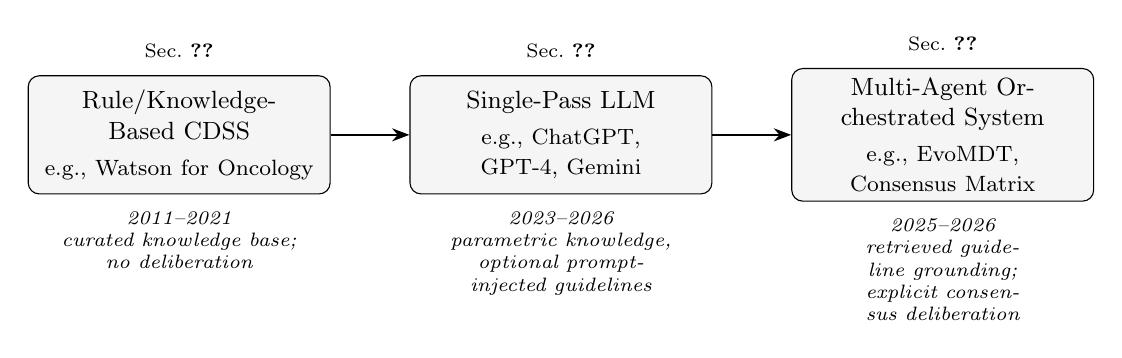
\begin{tikzpicture}[
  node distance=6mm and 10mm,
  gen/.style={draw, rounded corners, fill=gray!8, align=center, text width=3.6cm, minimum height=1.5cm, font=\small},
  lbl/.style={font=\scriptsize\itshape, align=center, text width=3.6cm},
  arr/.style={-{Stealth[length=2.2mm]}, thick}
]
\node[gen] (gen1) {Rule/Knowledge-Based CDSS\\[2pt]\footnotesize e.g., Watson for Oncology};
\node[lbl, below=1mm of gen1] (lbl1) {2011--2021\\curated knowledge base;\\no deliberation};

\node[gen, right=of gen1] (gen2) {Single-Pass LLM\\[2pt]\footnotesize e.g., ChatGPT, GPT-4, Gemini};
\node[lbl, below=1mm of gen2] (lbl2) {2023--2026\\parametric knowledge,\\optional prompt-injected guidelines};

\node[gen, right=of gen2] (gen3) {Multi-Agent Orchestrated System\\[2pt]\footnotesize e.g., EvoMDT, Consensus Matrix};
\node[lbl, below=1mm of gen3] (lbl3) {2025--2026\\retrieved guideline grounding;\\explicit consensus deliberation};

\draw[arr] (gen1) -- (gen2);
\draw[arr] (gen2) -- (gen3);

\node[font=\scriptsize, above=1mm of gen1] {Sec.~\ref{sec:rule-to-llm}};
\node[font=\scriptsize, above=1mm of gen2] {Sec.~\ref{sec:rule-to-llm}};
\node[font=\scriptsize, above=1mm of gen3] {Sec.~\ref{sec:multiagent-background}};
\end{tikzpicture}
\caption{Taxonomy of the three technological generations of AI-assisted tumor-board decision support identified in the literature reviewed (Sections~\ref{sec:rule-to-llm} and~\ref{sec:multiagent-background}). The generations emerged in sequence but, as Section~\ref{sec:trends} discusses, now coexist in the current literature rather than one fully displacing the last.}
\label{fig:taxonomy}
\end{figure}

\section{Thematic Literature Review}
\label{sec:thematic}

The 24 papers in the final literature set (methodology and tool comparison discussed in Section~\ref{sec:introduction} above) cluster into five overlapping themes: concordance between AI and human tumor-board decisions; multi-agent architectures for tumor-board simulation; implementation and operational models of virtual tumor boards; systematic and meta-analytic evidence; and cancer-type- or task-specific evaluations. Each is discussed in turn.

\subsection{Concordance Between AI/LLM Recommendations and Human Tumor-Board Decisions}
\label{sec:concordance}

Concordance studies are the largest and most methodologically consistent cluster in the literature: a set of retrospective or prospective cases previously discussed by a real MDT is re-presented to an AI system, and the two sets of recommendations are compared using the percentage-agreement statistic of Equation~\eqref{eq:concordance} or, less commonly, Cohen's kappa. Foundational work in this cluster used Watson for Oncology as the AI system under test. \citet{somashekhar2018} found 93\% concordance in breast cancer, with age and stage the strongest predictors of disagreement. The pattern generalizes: \citet{aliyev2026} find that concordance between MDT decisions and AI recommendations in endometrial cancer not only varies by case characteristics but that the direction of discordance (AI more aggressive vs.\ more conservative than the human board) is itself associated with different downstream clinical outcomes---a methodological advance over simple agreement-rate reporting, since it begins to connect concordance to patient-relevant consequences rather than treating disagreement as a single undifferentiated category. Table~\ref{tab:concordance} collects the headline concordance figures reported across this cluster and the related cancer-type-specific studies of Section~\ref{sec:cancer-specific}, to make the ``60\%--90\%'' range quoted in the Abstract concrete at the level of individual studies.

With the shift to LLMs, the same concordance paradigm was applied to ChatGPT and its successors across an increasing range of cancer types and clinical questions. \citet{ismayilov2025} simulate a full virtual tumor board using an LLM primed with National Cancer Institute guidelines for ten non-small-cell lung cancer (NSCLC) cases receiving immunotherapy, reporting high scores for content accuracy (4.9/5.0) and internal consistency (5.0/5.0), but noting that the model generated no recommendations beyond what the human MDT had already considered---a recurring limitation discussed further in Section~\ref{sec:challenges}. \citet{chatziisaak2025} evaluate ChatGPT on colorectal cancer MDT decisions, and \citet{ciulli2026} evaluate a generative AI model against a hepatobiliary MDT for hepatocellular carcinoma, both reporting moderate-to-substantial agreement with systematic disagreement concentrated in more complex, multi-modality treatment decisions. \citet{dogan2025} similarly report moderate ChatGPT--MDT agreement across mixed cancer-board decisions, framing their central question as whether an LLM should be considered a de facto ``member'' of the board rather than an external checker. \citet{pinninti2026} represent a methodological step forward within this cluster: a prospective, blinded, real-world concordance study comparing AI and MDT decision-making across multiple cancer types, rather than the retrospective, single-institution, single-cancer-type design that dominates the earlier literature. \citet{seshachalam2026} push this further still with a prospective blinded validation of LLM recommendations specifically against a molecular tumor board, framing their central finding as an ``AI paradox'': the model performs well on standardized, guideline-clear cases but its apparent reliability decreases precisely in the genomically complex cases where decision support would be most valuable---a finding that anticipates the ``complexity gap'' pattern formalized in the systematic-review literature (Section~\ref{sec:systematic}).

A methodological thread worth drawing out across this cluster is how the unit of comparison has narrowed over time. The earliest studies \citep{somashekhar2018} compared whole treatment plans against the tumor board's final decision, a coarse unit that conflates many independent sub-decisions (systemic therapy choice, surgical approach, radiation sequencing) into a single agree/disagree judgment. Later studies increasingly decompose this judgment: \citet{aliyev2026} separate agreement from the clinical direction of disagreement, and \citet{aubreville2024}---discussed further in Section~\ref{sec:cancer-specific}---narrows the target to a single procedural recommendation rather than a full treatment plan. This narrowing makes concordance figures from different points in the literature progressively harder to compare on a single scale, reinforcing the methodological-heterogeneity concern raised by the systematic reviews in Section~\ref{sec:systematic}.

\begin{table}[t]
\centering
\caption{Cross-study summary of reported AI-MDT concordance (Equation~\eqref{eq:concordance}), by representative study. ``Matching rule'' records whether the study used exact (top-choice) or broad (recommended-or-acceptable) agreement, since Section~\ref{sec:challenges} argues this materially affects comparability across rows.}
\label{tab:concordance}
\small
\begin{tabular}{P{2.4cm}P{1.6cm}P{2.6cm}P{1.6cm}P{2.9cm}}
\toprule
\textbf{Study} & \textbf{AI class} & \textbf{Cancer type / setting} & \textbf{Matching rule} & \textbf{Reported concordance} \\
\midrule
\citet{somashekhar2018} & Rule/CDSS & Breast (638 cases) & Exact & 93\% \\
\citet{park2023} & Rule/CDSS & Gastric (322 cases) & Broad & 86.96\% (72.98\% exact) \\
\citet{wu2026} & Systematic review & Surgical oncology (59 studies) & Mixed & 23--99\% range \\
\citet{wang2025iscience} & Review synthesis & Mixed cancers (narrative review) & Mixed & 70--90\% typical range \\
\citet{ismayilov2025} & Single-pass LLM & NSCLC, immunotherapy (10 cases) & Rating scale & 4.9/5.0 content accuracy \\
\citet{chatziisaak2025} & Single-pass LLM & Colorectal & Broad & Moderate--substantial agreement \\
\citet{ciulli2026} & Single-pass LLM & Hepatocellular carcinoma & Broad & Moderate--substantial agreement \\
\citet{aliyev2026} & Single-pass LLM & Endometrial & Broad, direction-coded & Varies by case; direction linked to outcomes \\
\citet{liu2026} & Multi-agent (EvoMDT) & Multi-cancer (benchmarks + pilot) & Physician review & Comparable to human MDT; 30--40\% faster \\
\citet{pinninti2026} & Single-pass LLM & Multi-cancer & Prospective, blinded & Reported as high; first multi-cancer prospective design \\
\citet{seshachalam2026} & Single-pass LLM & Molecular tumor board & Prospective, blinded & High on standard cases; declines on complex cases (``AI paradox'') \\
\bottomrule
\end{tabular}
\end{table}

\subsection{Multi-Agent Architectures for Tumor-Board Simulation}
\label{sec:multiagent}

A second, more recent cluster of papers moves beyond single-LLM concordance testing to propose and evaluate architectures that explicitly distribute reasoning across multiple coordinated agents. EvoMDT \citep{liu2026} is the most fully evaluated example in this review: benchmarked across six public oncology question-answering datasets and four real-world datasets spanning breast, liver, lung, and lymphoma cancers, it outperforms frontier LLM baselines (including Llama-3-70B, Claude-3, and Med-PaLM~2) on guideline concordance and semantic alignment with expert plans, and in physician review achieves decision quality comparable to human MDTs while reducing response time by 30--40\%. \citet{wang2025jco} propose a ``virtual oncology collaborative tumor board'' built from multiple AI agents, directly modeling the collaborative structure of a real MDT rather than a single input-output prediction task. \citet{han2025} contribute a ``Multi-Agent Medical Decision Consensus Matrix System,'' formalizing how individual agent outputs are aggregated into a collective recommendation---addressing a gap left open by earlier single-LLM studies, which have no principled mechanism for resolving disagreement when multiple model outputs are generated. \citet{saenz2026} and \citet{kuerbanjiang2025} extend multi-agent, guideline-grounded architectures to hepatocellular carcinoma and complex gynecologic oncology respectively, suggesting the approach generalizes across cancer types rather than being specific to the datasets on which it was first demonstrated. Table~\ref{tab:multiagent} (Section~\ref{sec:comparison}) compares these five systems directly along the design axes introduced in Section~\ref{sec:multiagent-background}.

Across this cluster, three recurring design elements distinguish multi-agent systems from single-LLM concordance studies: (1) explicit guideline or knowledge retrieval, grounding agent outputs in current clinical evidence rather than relying solely on parametric model knowledge; (2) a consensus or deliberation mechanism that resolves disagreement between agents, analogous to the negotiation that occurs in a real MDT meeting; and (3) evaluation against structured, traceable outputs (evidence-linked recommendations) rather than a single free-text recommendation, which improves auditability but also raises the bar for what counts as a ``correct'' answer. These design choices position multi-agent systems as the closest AI analogue yet developed to the deliberative structure of a human tumor board, though---as discussed in Section~\ref{sec:challenges}---prospective, patient-outcome-linked validation of these architectures remains largely absent from the literature reviewed here.

It is also notable how recently this entire cluster has appeared. With the exception of early consensus-modeling work outside the immediate tumor-board context, every multi-agent paper in this review's literature set was published in 2025 or 2026 (Figure~\ref{fig:taxonomy}), meaning the field has had, at most, one to two years to accumulate independent replication or long-term follow-up. This recency should temper how the strong headline results---particularly EvoMDT's reported parity with human MDT decision quality---are read: they represent the current best evidence for what multi-agent orchestration can achieve, not yet a settled, externally validated finding.

\subsection{Implementation and Operational Models of Virtual Tumor Boards}
\label{sec:implementation}

A distinct, earlier-established cluster of literature addresses VTBs as an operational and access-to-care intervention, independent of AI decision support. \citet{marshall2014} and \citet{thiagarajan2023}---discussed above as conceptual anchors in Section~\ref{sec:mdt-vtb}---establish that VTBs are feasible, well accepted by participating clinicians, and effective at extending specialist reach into settings that would otherwise lack access to multidisciplinary review; in the Thiagarajan et al.\ cohort, 96.1\% of participating centers agreed with the VTB's decisions and a similar proportion rated the sessions a useful educational platform. \citet{patkar2011}, though it predates the ``virtual'' framing specifically, provides the evidentiary basis for why MDTs (and by extension VTBs) matter clinically: guideline adherence, documentation quality, and coordination of care are consistently improved by structured multidisciplinary review, even where direct survival benefit is harder to establish.

This implementation-focused cluster is thematically important to the present review for two reasons. First, it supplies the operational baseline against which AI-augmented VTBs must be judged: any AI system proposed for tumor-board use is competing not against an idealized decision process but against the real logistical and cognitive constraints of the meetings described in this literature---time pressure, incomplete information at presentation, and variable case documentation. Second, it highlights that the ``virtual'' and the ``AI-assisted'' aspects of a tumor board are conceptually separable and were historically developed on different timelines: VTBs as a telemedicine intervention predate LLM-based decision support by roughly a decade, and the concordance and multi-agent literature reviewed in Sections~\ref{sec:concordance} and~\ref{sec:multiagent} is best understood as a second wave of innovation layered onto an already-established virtual-meeting infrastructure, rather than a simultaneous, co-designed development.

\subsection{Systematic Reviews and Meta-Analytic Evidence}
\label{sec:systematic}

Four systematic reviews and one meta-analysis in the literature set consolidate the primary-study evidence discussed above and are the source of this review's central cross-cutting claim: reported AI-MDT concordance is highly heterogeneous across studies, and that heterogeneity is not fully explained by cancer type alone. \citet{jie2021} meta-analyze Watson for Oncology's clinical application specifically, providing the most rigorous quantitative synthesis available for the pre-LLM era. \citet{oehring2023} systematically review the broader class of AI-based decision support systems for tumor diseases (not limited to WFO), reporting substantial variation in both the accuracy and evaluation methodology used across included studies---a methodological critique that generalizes to the LLM-era literature reviewed here. \citet{carl2024} and \citet{wu2026} extend this synthesis into the LLM and multi-agent era specifically. \citet{carl2024} review 34 studies of LLM use in clinical oncology broadly (not limited to tumor boards) and report significant performance variance attributable to differences in prompting strategy, model choice, and evaluation criteria, concluding that the field lacks standardized, LLM-specific reporting protocols---a direct methodological gap this review's Section~\ref{sec:challenges} returns to. \citet{wu2026}, reviewing 59 studies specifically in surgical oncology MDT decision-making, is the most comprehensive single synthesis in the literature set: it classifies AI-CDSS approaches into the five-category taxonomy introduced in Section~\ref{sec:rule-to-llm}, reports the 23--99\% concordance range cited throughout this review, and---notably---is the only systematic review in the set to explicitly name implementation barriers (system maintenance burden, variability in clinical protocols across institutions, and treatment-accessibility differences) as a first-order finding alongside accuracy figures, rather than treating them as a secondary caveat. \citet{konzmann2026} contribute a fourth, more recent systematic review focused specifically on LLM applications in tumor boards, corroborating the pattern that guideline grounding and consensus deliberation---rather than raw model scale---are the design features most associated with higher reported concordance in the 2025--2026 literature.

\subsection{Cancer-Type- and Task-Specific Evaluations}
\label{sec:cancer-specific}

A final cluster comprises studies that apply the concordance or multi-agent paradigm to a specific cancer type or clinical task not otherwise represented, and collectively demonstrate the breadth of settings in which the underlying AI-MDT question has now been tested: gastric cancer \citep{park2023}, gynecologic oncology \citep{kuerbanjiang2025}, hepatocellular carcinoma \citep{saenz2026,ciulli2026}, endometrial cancer \citep{aliyev2026}, colorectal cancer \citep{chatziisaak2025}, mixed cancer boards \citep{dogan2025}, and head-and-neck cancer procedural planning specifically \citep{aubreville2024}. \citet{park2023} is a particularly detailed example within this cluster: in a retrospective analysis of 322 gastric-cancer cases at a single Korean center, WFO--MTB concordance was 86.96\% under a broad matching rule (72.98\% under strict matching), but fell to 45.83\% in Stage~IV disease---age, performance status, and advanced stage were all independently associated with lower concordance, illustrating the complexity-gap pattern (Section~\ref{sec:challenges}) at the level of individual patient covariates rather than only cancer type. \citet{aubreville2024} is methodologically distinct within this cluster: rather than testing whole-case treatment concordance, it evaluates whether an LLM can predict the specific procedural recommendation a tumor board will make, narrowing the prediction task in a way that may be more tractable for near-term clinical deployment than full treatment-plan generation. Taken together, this cluster suggests the field is moving toward the kind of cancer-type-by-cancer-type validation that a genuinely generalizable clinical AI system would eventually require, even though---as Section~\ref{sec:gaps} discusses---no single study in this review validates a system across more than a handful of cancer types simultaneously.

\section{Comparison of Existing Approaches}
\label{sec:comparison}

The literature reviewed above reflects three broadly distinct technical approaches to AI-assisted tumor-board decision support, which emerged in sequence (Figure~\ref{fig:taxonomy}) but now coexist in the current literature: rule- and knowledge-based clinical decision support systems, single-pass large language models, and multi-agent orchestrated systems. Table~\ref{tab:comparison} compares these approaches along the dimensions most consistently reported across the reviewed studies.

\begin{table}[t]
\centering
\caption{Comparison of the three major classes of AI approach to tumor-board decision support identified in the literature.}
\label{tab:comparison}
\small
\begin{tabular}{P{2.2cm}P{3.3cm}P{3.5cm}P{3.5cm}}
\toprule
\textbf{Dimension} & \textbf{Rule/Knowledge-Based CDSS} (e.g., Watson for Oncology) & \textbf{Single-Pass LLM} (e.g., ChatGPT, GPT-4, Gemini) & \textbf{Multi-Agent Orchestrated System} (e.g., EvoMDT, Consensus Matrix) \\
\midrule
Representative studies & \citet{somashekhar2018}; \citet{jie2021} (meta-analysis) & \citet{ismayilov2025}; \citet{chatziisaak2025}; \citet{ciulli2026}; \citet{aliyev2026} & \citet{liu2026} (EvoMDT); \citet{han2025}; \citet{saenz2026}; \citet{wang2025jco}; \citet{kuerbanjiang2025} \\
Knowledge source & Curated, expert-annotated knowledge base & Parametric model knowledge, optionally supplemented by prompt-injected guidelines & Retrieved, guideline-grounded evidence plus parametric knowledge, distributed across agents \\
Deliberation structure & None --- single recommendation output & None --- single-pass recommendation, occasionally re-queried & Explicit multi-agent consensus/deliberation protocol analogous to MDT negotiation \\
Typical evaluation design & Retrospective, single-institution concordance & Retrospective, single- or few-institution concordance; occasional prospective pilot & Benchmark datasets plus retrospective/pilot concordance; prospective validation rare \\
Reported concordance range & $\sim$85--93\% in flagship studies; lower in edge cases \citep{somashekhar2018} & $\sim$56--87\% depending on cancer type and case complexity \citep{aliyev2026,chatziisaak2025} & Comparable to human MDT decision quality in the best-evaluated system \citep{liu2026}, with 30--40\% faster response \\
Principal strength & Stable, auditable, guideline-curated outputs & Low deployment barrier; flexible across case types without system-specific engineering & Closest structural analogue to real MDT deliberation; traceable, evidence-linked outputs \\
Principal limitation & Costly to build and maintain; brittle outside curated scope \citep{wu2026} & Hallucination and inconsistency risk; no mechanism to resolve internal disagreement & Architecturally complex; least mature evidence base; prospective validation largely absent \\
\bottomrule
\end{tabular}
\end{table}

As shown in Table~\ref{tab:comparison}, no single approach dominates across all dimensions. Rule-based systems remain the most extensively validated in aggregate concordance terms, largely because they have been studied longest, but \citet{wu2026} and \citet{oehring2023} both note that this maturity comes at the cost of high development and maintenance burden, and that performance degrades sharply outside the system's curated scope. Single-pass LLMs lower the barrier to running a concordance study dramatically---most studies in this cluster required no more infrastructure than a case summary and a chat interface---but this same simplicity means they cannot represent the division of expertise or internal disagreement resolution that characterizes a real tumor board; \citet{ismayilov2025} explicitly note that their LLM-simulated board generated no insight beyond what the human MDT had already produced. Multi-agent systems are designed specifically to recover that missing deliberative structure, and the single best-documented example (EvoMDT) reports the strongest results of any system reviewed on both concordance and efficiency measures. However, this class of system is also the newest and least externally validated: with the partial exception of EvoMDT's multi-dataset benchmarking, none of the multi-agent studies in this review report the kind of prospective, multi-institutional, blinded validation that \citet{pinninti2026} and \citet{seshachalam2026} have begun to establish as the emerging standard for single-LLM concordance work.

Table~\ref{tab:multiagent} narrows the focus to the multi-agent cluster itself (Section~\ref{sec:multiagent}), comparing the five systems on the three design axes introduced in Section~\ref{sec:multiagent-background}: guideline retrieval, an explicit consensus mechanism, and the maturity of the evaluation performed.

\begin{table}[t]
\centering
\caption{Architectural comparison of the multi-agent systems reviewed in Section~\ref{sec:multiagent}, along the design axes introduced in Section~\ref{sec:multiagent-background}.}
\label{tab:multiagent}
\small
\begin{tabular}{P{2.1cm}P{1.9cm}P{1.6cm}P{1.9cm}P{2.9cm}}
\toprule
\textbf{System} & \textbf{Cancer scope} & \textbf{Guideline retrieval} & \textbf{Consensus mechanism} & \textbf{Evaluation maturity} \\
\midrule
EvoMDT \citep{liu2026} & Multi-cancer (breast, liver, lung, lymphoma) & Yes, structured knowledge retrieval & Self-evolving consensus protocol with outcome feedback & Strongest: 6 QA benchmarks + 4 real-world datasets + physician review \\
Consensus Matrix \citep{han2025} & Not cancer-specific (general oncology MDT) & Partial & Explicit consensus-matrix aggregation of agent outputs & Architecture proposal; limited external validation reported \\
Guideline-grounded MA \citep{saenz2026} & Hepatocellular carcinoma & Yes, explicit guideline retrieval & Multi-agent deliberation & Single cancer type; retrospective/pilot \\
Virtual Collaborative Board \citep{wang2025jco} & Not cancer-specific & Partial & Multi-agent collaborative structure modeling MDT roles & Architecture proposal; limited external validation reported \\
Gynecologic MA Teams \citep{kuerbanjiang2025} & Gynecologic oncology & Yes & Multi-agent team deliberation & Single cancer type; preprint-stage evidence \\
\bottomrule
\end{tabular}
\end{table}

Table~\ref{tab:multiagent} makes explicit what Section~\ref{sec:multiagent} argues in prose: EvoMDT is the only system in this cluster evaluated against both public benchmarks and independent real-world datasets with physician review, while the remaining four systems are, at the time of this review, architecture proposals validated on a single cancer type or with preprint-stage evidence. This asymmetry is itself a research gap (Section~\ref{sec:gaps}): the field currently has one well-evaluated exemplar and several plausible but thinly validated variants, rather than a body of comparably rigorous multi-agent evidence.

\section{Research Trends / Developments}
\label{sec:trends}

Three trends are visible across the publication timeline of the reviewed literature. First, there is a clear generational shift in the underlying technology under study, consistent with the taxonomy in Figure~\ref{fig:taxonomy}: rule-based CDSS papers cluster in 2018--2021 \citep{somashekhar2018,jie2021}, single-LLM concordance papers cluster in 2023--2026 and now dominate the volume of new publications, and multi-agent architecture papers are concentrated almost entirely in 2025--2026 \citep{liu2026,han2025,saenz2026,wang2025jco}, indicating that multi-agent orchestration is the current frontier of the field rather than an established, mature approach.

Second, evaluation methodology is visibly maturing, even within the LLM-concordance cluster alone. The earliest LLM studies in this review are retrospective, single-institution, and unblinded case-comparison designs. \citet{pinninti2026} and \citet{seshachalam2026}---both published toward the end of the period covered---represent a methodological step change toward prospective, blinded, and in Pinninti et al.'s case multi-cancer-type designs, addressing a limitation that the systematic reviews \citep{carl2024,wu2026} explicitly identify as a weakness of the earlier literature. This suggests the field is self-correcting toward higher evidentiary standards as it matures, though prospective designs remain a minority of the total literature reviewed.

Third, the object of evaluation is broadening from ``does the AI agree with the tumor board'' toward more granular and more clinically situated questions: discordance direction and its association with outcomes \citep{aliyev2026}, task-specific procedural-recommendation prediction rather than whole-case treatment planning \citep{aubreville2024}, patient-covariate-level concordance analysis \citep{park2023}, and multi-cancer-type generalization within a single study \citep{liu2026,pinninti2026}. This broadening mirrors the trajectory that earlier, non-AI VTB implementation research followed a decade prior---from ``is this feasible'' \citep{marshall2014} toward ``how does this operate at scale and in what settings'' \citep{thiagarajan2023}---suggesting a recognizable maturation pattern common to both waves of tumor-board innovation.

\section{Challenges and Limitations}
\label{sec:challenges}

The literature reviewed here shares a set of recurring challenges that appear across nearly every technical approach and cancer type studied.

\textbf{Methodological heterogeneity and non-comparability.} \citet{carl2024} and \citet{wu2026} both identify a lack of standardized, LLM-specific reporting protocols as a fundamental barrier to comparing results across studies: differences in prompting strategy, case-selection criteria, concordance definitions (recall the exact-vs.-broad matching-rule distinction formalized in Equation~\eqref{eq:concordance} and illustrated concretely in Table~\ref{tab:concordance}), and rater blinding mean that a reported concordance figure from one study is frequently not directly comparable to another, even within the same cancer type. This is compounded by small, single-institution sample sizes in the majority of primary studies reviewed (commonly 10--100 cases, though \citet{park2023} and \citet{somashekhar2018} are notable larger-cohort exceptions at 322 and 638 cases respectively), which limits statistical power and generalizability.

\textbf{The ``complexity gap.''} A pattern recurring across nearly every concordance study is that AI performance is strongest on standardized, guideline-clear, high-incidence cases (e.g., early-stage breast or gynecologic cancer) and degrades in rare, multimodal, or genomically complex cases---precisely the scenarios in which clinical decision support would be most valuable. This pattern is explicit in \citeauthor{seshachalam2026}'s \citeyearpar{seshachalam2026} ``AI paradox'' framing, in \citeauthor{wu2026}'s \citeyearpar{wu2026} 23--99\% concordance range, in the Stage-IV concordance collapse (86.96\% overall to 45.83\% in Stage~IV) reported by \citet{park2023}, and implicit in the stage-dependent concordance decline reported by \citet{somashekhar2018} nearly a decade earlier---indicating the complexity gap is not specific to any one generation of AI technology (Table~\ref{tab:concordance} makes this pattern visible across studies at a glance).

\textbf{Safety, hallucination, and lack of internal disagreement resolution.} Single-pass LLMs carry a documented risk of fabricated or misapplied guideline citations and inconsistent recommendations across repeated queries, and---unlike a real MDT or a multi-agent system with an explicit consensus mechanism---have no internal process for surfacing or resolving their own uncertainty. Multi-agent systems are designed to address this specific limitation, but their added architectural complexity introduces new failure surfaces (e.g., errors in how individual agent outputs are weighted or reconciled) that are not yet well characterized in the literature reviewed here, as Table~\ref{tab:multiagent}'s evaluation-maturity column also suggests.

\textbf{Absence of patient-outcome-linked validation.} With the partial exception of \citet{aliyev2026}, who link discordance direction to downstream clinical outcomes, every study in this review evaluates AI systems against tumor-board recommendations, not against measured patient outcomes such as survival, recurrence, or quality of life. This means the field currently has robust evidence that AI can approximate what a tumor board would recommend, but very limited evidence on whether AI-assisted recommendations lead to better, equivalent, or worse patient outcomes than unassisted human decision-making.

\textbf{Implementation and integration barriers.} \citet{wu2026} is notable for treating system maintenance burden, cross-institutional protocol variability, and treatment-accessibility differences as first-order findings rather than caveats. These barriers---electronic health record integration, clinician trust and workflow disruption, and the governance and regulatory questions raised by using AI-generated recommendations in real treatment decisions---are acknowledged across the reviewed literature but are rarely the primary object of study, representing an important gap discussed further below.

\section{Research Gaps}
\label{sec:gaps}

Several gaps emerge consistently from the thematic synthesis above. First, prospective, multi-institutional, randomized or blinded validation remains rare: only \citet{pinninti2026} and \citet{seshachalam2026} in this review employ prospective, blinded designs, and neither is a randomized controlled trial. Second, no study in the reviewed literature links AI-assisted or multi-agent-assisted tumor-board recommendations to measured patient outcomes; the field's evidence base stops at recommendation-level concordance. Third, standardized, cross-study concordance metrics and reporting protocols do not exist, which---as \citet{carl2024} argue---makes it difficult to determine whether reported performance differences between studies reflect genuine differences in system capability or simply differences in evaluation methodology (the matching-rule column of Table~\ref{tab:concordance} is one symptom of this problem). Fourth, multi-agent systems, despite showing the strongest reported results \citep{liu2026}, have the thinnest independent validation: as Table~\ref{tab:multiagent} shows directly, four of the five reviewed architectures are evaluated by their own developers on datasets the same team assembled, and cross-institutional replication of multi-agent results is absent from this review's literature set. Fifth, representation of low- and middle-income-country contexts is limited to VTB implementation studies \citep{thiagarajan2023} rather than AI-augmented VTB studies specifically, leaving open whether the concordance and efficiency gains reported in the high-resource settings studied here would generalize to the resource-constrained settings where VTB access gains are arguably most needed. Finally, the literature is almost silent on cost-effectiveness, clinician workload impact, and medico-legal or governance frameworks for deploying AI recommendations in an actual tumor-board setting---questions that will determine real-world adoption independently of concordance accuracy.

\section{Future Research Directions}
\label{sec:future}

Building directly on the gaps identified above, five directions appear most likely to advance the field. First, prospective, multi-institutional, outcome-linked studies that follow patients beyond the point of recommendation to measure the real clinical consequence of AI-assisted versus unassisted tumor-board decisions, building on the discordance-outcome linkage that \citet{aliyev2026} has begun to establish. Second, the development of standardized concordance-reporting protocols---analogous to CONSORT or STARD reporting guidelines in other areas of clinical AI research, and explicitly anchored to a single formal definition such as Equation~\eqref{eq:concordance} together with a declared matching rule---that would make cross-study comparison meaningful, a need explicitly flagged by \citet{carl2024}. Third, independent, cross-institutional replication of multi-agent architectures such as EvoMDT and the Consensus Matrix system, evaluated on data and by teams independent of the original developers, to establish whether their strong reported results generalize; Table~\ref{tab:multiagent} identifies exactly which of the five reviewed systems most urgently need this replication. Fourth, multimodal extension of both single-LLM and multi-agent systems to directly incorporate imaging, pathology, and genomic data rather than relying on text case summaries alone, addressing a limitation implicit throughout the reviewed concordance literature and explicit in the ``complexity gap'' pattern. Fifth, deployment-focused research on workflow integration, clinician trust calibration, and governance frameworks---extending \citeauthor{wu2026}'s \citeyearpar{wu2026} identification of implementation barriers into a dedicated research program rather than a secondary finding---alongside economic evaluation of whether AI-assisted VTBs reduce the specialist-time burden that motivated the entire line of research in the first place.

\section{Conclusion}
\label{sec:conclusion}

This review synthesized 24 papers on AI- and multi-agent-assisted virtual tumor boards, drawn from Semantic Scholar, ResearchRabbit, Litmaps, and Elicit, spanning fifteen years of research from the earliest VTB implementation studies through the current generation of multi-agent, guideline-grounded decision-support architectures. The evidence base shows a clear technological progression---from rule-based clinical decision support, through single-pass large language models, to multi-agent orchestrated systems (Figure~\ref{fig:taxonomy})---and a parallel, if less complete, methodological progression from retrospective, single-institution concordance studies toward prospective, blinded, multi-cancer-type validation. Reported AI-MDT concordance (Equation~\eqref{eq:concordance}, Table~\ref{tab:concordance}) is consistently high on standardized cases and consistently weaker on rare or complex ones, a ``complexity gap'' that recurs across every technical generation studied and that current multi-agent architectures (Table~\ref{tab:multiagent}) are designed, but not yet independently proven, to close. The most significant open question is not whether AI can approximate a tumor board's recommendation---the accumulated concordance evidence suggests it often can---but whether AI-assisted deliberation improves the outcomes that tumor boards exist to protect, a question this literature has not yet been designed to answer. Prospective, outcome-linked, multi-institutional research, paired with standardized reporting and independent replication of the newest multi-agent architectures, represents the clearest path from the current concordance-focused evidence base to clinically actionable conclusions about the role of AI in the virtual tumor board.

\bibliographystyle{ACM-Reference-Format}
\bibliography{references}

\end{document}
